% Môn: Vật lý
% Lớp: 12
% Chương: Chương I. Vật lí nhiệt
% Bài: L12C1 Bài 6. Nhiệt hóa hơi riêng · Giải thích hiện tượng thực tế liên quan đến chuyển thể
% ID: L12C1B1-TN-42
% Mức: NB
% ID: L12C1B1-91-TN


% ID: L12C1B1-TN-37
% Mức: TH
% ID: L12C1B1-104-TN
% ID: L12C1B1-104-TN
% Mức: TH
% ID: L12C1B6-62-TN
%=== Câu 14 ===%
\dangbt{Giải thích hiện tượng thực tế liên quan đến chuyển thể}
\begin{ex}
% ID: L12C1B6-62-TN
% Mức: TH
	{\color{red}\footnotesize\ttfamily [L12C1B1-TN-37]}\par %HienID
	Những quá trình chuyển thể nào của đồng được vận dụng trong việc đúc tượng đồng?
	\choice
	{\True Nóng chảy và đông đặc}
	{Nóng chảy và bay hơi}
	{Bay hơi và ngưng tụ}
	{Bay hơi và đông đặc}
	\loigiai{
		\begin{itemize}
			\item Quá trình chuyển thể được vận dụng trong việc đúc tượng đồng là nóng chảy và đông đặc.
		\end{itemize}
	}
\end{ex}

% ID: L12C1B1-TN-40
% Mức: VD
% ID: L12C1B1-106-TN
% ID: L12C1B1-106-TN
% Mức: VD
% ID: L12C1B6-63-TN
%=== Câu 16 ===%
\begin{ex}
% ID: L12C1B6-63-TN
% Mức: VD
	{\color{red}\footnotesize\ttfamily [L12C1B1-TN-40]}\par %HienID
	Các bình hình bên đều đựng cùng một lượng nước. Để cả ba bình vào trong phòng kín. Hỏi sau một tuần bình nào còn ít nước nhất?
	\begin{center}
		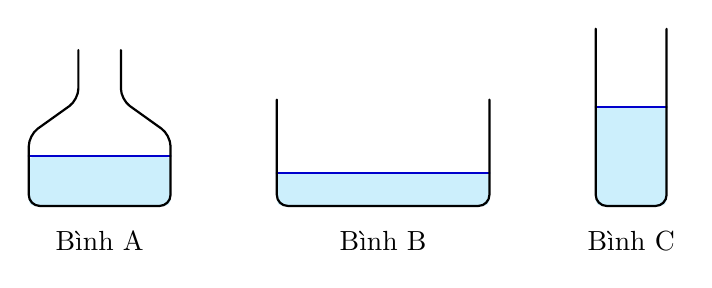
\begin{tikzpicture}[
			line join=round,
			line cap=round,
			scale=0.9,
			bo/.style={rounded corners=4pt},
			nuoc/.style={cyan!20, rounded corners=2pt}
			]
			\begin{scope}[shift={(0,0)}]
				\fill[nuoc] (0,0) rectangle (2,0.7);
				\draw[blue!80!black, thick] (0,0.7) -- (2,0.7);
				\draw[thick, bo]
				(0.7,2.2) -- (0.7,1.5) -- (0,1) -- (0,0)
				-- (2,0) -- (2,1) -- (1.3,1.5) -- (1.3,2.2);
				\node at (1,-0.5) {Bình A};
			\end{scope}
			\begin{scope}[shift={(3.5,0)}]
				\fill[nuoc] (0,0) rectangle (3,0.47);
				\draw[blue!80!black, thick] (0,0.47) -- (3,0.47);
				\draw[thick, bo]
				(0,1.5) -- (0,0) -- (3,0) -- (3,1.5);
				\node at (1.5,-0.5) {Bình B};
			\end{scope}
			\begin{scope}[shift={(8,0)}]
				\fill[nuoc] (0,0) rectangle (1,1.4);
				\draw[blue!80!black, thick] (0,1.4) -- (1,1.4);
				\draw[thick, bo]
				(0,2.5) -- (0,0) -- (1,0) -- (1,2.5);
				\node at (0.5,-0.5) {Bình C};
			\end{scope}
		\end{tikzpicture}
	\end{center}
	\choice
	{Bình A}
	{\True Bình B}
	{Bình C}
	{Chưa xác định được}
	\loigiai{
		\begin{itemize}
			\item Cả ba bình đều để trong cùng điều kiện về nhiệt độ, áp suất, độ ẩm, …
			\item Tốc độ bay hơi của nước phụ thuộc vào diện tích mặt thoáng.
			\item Bình B có diện tích mặt thoáng lớn nhất nên nước bay hơi nhiều nhất và sẽ còn lại ít nhất.
		\end{itemize}
	}
\end{ex}

% ID: L12C1B1-TN-8
% Mức: TH
% ID: L12C1B1-110-TN
% ID: L12C1B1-110-TN
% Mức: TH
% ID: L12C1B6-64-TN
%=== Câu 20 ===%
\begin{ex}
% ID: L12C1B6-64-TN
% Mức: TH
	{\color{red}\footnotesize\ttfamily [L12C1B1-TN-8]}\par %HienID
	Đầu năm $2\,024$, các quốc gia Bắc Âu đã chứng kiến thời tiết cực lạnh, với nhiệt độ thấp nhất trong $25$ năm ở mức $-44{,}3^\circ \mathrm{C}$, người dân đã đun sôi nước, nhanh chóng mang ra ngoài và hất tung nó theo hình vòng cung trên không trung, ngay lập tức biến thành một đám mây băng giá. Đây là hiện tượng
	\choice
	{ngưng kết}
	{\True đông đặc}
	{ngưng tụ}
	{nóng chảy}
	\loigiai{
		\begin{itemize}
			\item Người dân đã đun sôi nước, nhanh chóng mang ra ngoài và hất tung nó theo hình vòng cung trên không trung, ngay lập tức biến thành một đám mây băng giá đây là hiện tượng đông đặc.
		\end{itemize}
	}
\end{ex}

% ID: L12C1B1-TN-11
% Mức: TH
% ID: L12C1B1-112-TN
% ID: L12C1B1-112-TN
% Mức: TH
% ID: L12C1B6-65-TN
%=== Câu 22 ===%
\begin{ex}
% ID: L12C1B6-65-TN
% Mức: TH
	{\color{red}\footnotesize\ttfamily [L12C1B1-TN-11]}\par %HienID
	Tình huống nào sau đây \textbf{không}  liên quan đến hiện tượng nóng chảy?
	\choice
	{Đốt một ngọn nến}
	{Đun nấu mỡ vào mùa đông}
	{Pha nước chanh đá}
	{\True Cho nước vào tủ lạnh để làm đá}
	\loigiai{
		Tình huống không liên quan đến hiện tượng nóng chảy là cho nước vào tủ lạnh để làm đá.}
\end{ex}

% ID: L12C1B1-TN-13
% Mức: TH
% ID: L12C1B1-114-TN
% ID: L12C1B1-114-TN
% Mức: TH
% ID: L12C1B6-66-TN
%=== Câu 24 ===%
\begin{ex}
% ID: L12C1B6-66-TN
% Mức: TH
	{\color{red}\footnotesize\ttfamily [L12C1B1-TN-13]}\par %HienID
	Tình huống \textbf{không} liên quan đến hiện tượng nóng chảy là
	\choice
	{đốt một ngọn nến}
	{đun nấu mỡ vào mùa đông}
	{pha nước chanh đá}
	{\True cho nước vào tủ lạnh để làm nước đá}
	\loigiai{- Sự nóng chảy là sự chuyển từ thể rắn sang thể lỏng
		- Cho nước vào tủ lạnh để làm đá là sự chuyển từ thể lỏng sang thể rắn
	}
\end{ex}

% ID: L12C1B1-TN-14
% Mức: TH
% ID: L12C1B1-115-TN
% ID: L12C1B1-115-TN
% Mức: TH
% ID: L12C1B6-67-TN
%=== Câu 25 ===%
\begin{ex}
% ID: L12C1B6-67-TN
% Mức: TH
	{\color{red}\footnotesize\ttfamily [L12C1B1-TN-14]}\par %HienID
	Nhiệt độ đông đặc của rượu là $-117^\circ \mathrm{C}$, của thủy ngân là $-38{,}83^\circ \mathrm{C}$. Ở nước lạnh người ta dùng \choice
	{nhiệt kế thủy ngân vì nhiệt kế thủy ngân rất chính xác}
	{nhiệt kế thủy ngân vì nhiệt độ đông đặc của thủy ngân cao hơn nhiệt độ đông đặc của rượu}
	{nhiệt kế thủy ngân vì ở âm vài chục $^\circ \mathrm{C}$ rượu bay hơi hết}
	{\True nhiệt kế rượu vì nhiệt kế rượu có thể đo nhiệt độ môi trường $-50^\circ \mathrm{C}$}
	\loigiai{Nhiệt độ đông đặc của rượu thấp hơn nhiệt độ đông đặc của thủy ngân rất nhiều nên ở nước lạnh người ta dùng nhiệt kế rượu để đo nhiệt độ của môi trường khi nhiệt độ giảm xuống âm vài chục°C}
\end{ex}

% ID: L12C1B1-TN-19
% Mức: VD
% ID: L12C1B1-118-TN
% ID: L12C1B1-118-TN
% Mức: VD
% ID: L12C1B6-68-TN
%=== Câu 28 ===%
\begin{ex}
% ID: L12C1B6-68-TN
% Mức: VD
	{\color{red}\footnotesize\ttfamily [L12C1B1-TN-19]}\par %HienID
	Thành phần chính của gang là sắt, ngoài ra còn các nguyên liệu khác là carbon và silic tồn tại ở trạng thái đông đặc. Để chế tạo gang, một người thợ nấu chảy mẻ thép phế liệu trong một chiếc nồi kim loại đặc biệt và người đó bỏ thêm vào nồi thép nóng chảy đỏ rực đó một ít rơm khô. Để không bị hòa tan với thép nóng chảy thì kim loại làm nồi nấu phải có
	\choice
	{nhiệt độ hóa hơi cao hơn nhiệt độ hóa hơi của gang và thép}
	{nhiệt độ nóng chảy thấp hơn nhiệt độ hóa hơi của gang và thép}
	{nhiệt độ ngưng kết thấp hơn nhiệt độ hóa hơi của gang và thép}
	{\True nhiệt độ nóng chảy cao hơn nhiệt độ hóa hơi của gang và thép}
	\loigiai{Để nấu chảy gang và thép, nồi nấu phải có nhiệt độ nóng chảy cao hơn nhiệt độ nóng chảy của gang và thép để tránh bị tan chảy trong quá trình sử dụng. Cần đảm bảo tính ổn định và bền vững của nồi nấu trong môi trường nhiệt độ cao.}
\end{ex}

% ID: L12C1B1-TN-21
% Mức: VD
% ID: L12C1B1-120-TN
% ID: L12C1B1-120-TN
% Mức: VD
% ID: L12C1B6-69-TN
%=== Câu 30 ===%
\begin{ex}
% ID: L12C1B6-69-TN
% Mức: VD
	{\color{red}\footnotesize\ttfamily [L12C1B1-TN-21]}\par %HienID
	\immini{
		Nồi áp suất có cơ chế điều chỉnh giải phóng hơi nước để duy trì áp suất không đổi. Nồi đang sôi, nếu cơ chế đó bị tắc thì}
	{		
		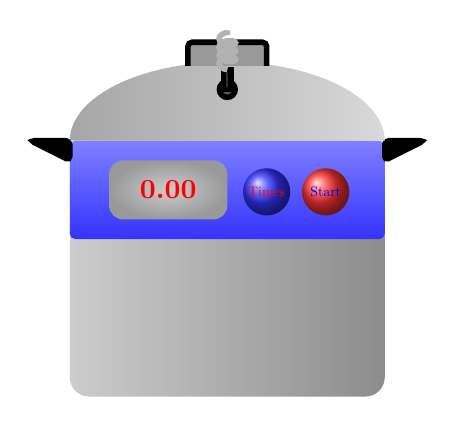
\begin{tikzpicture}[line width=2pt, scale=0.5]
			
			\shade[left color=gray!40, right color=gray!90, rounded corners=7pt] 
			(-4,-4) rectangle (4,2.5);
			
			\shade[top color=blue!50, bottom color=blue!80, rounded corners=2pt] 
			(-4,0) rectangle (4,2.5);
			
			\draw[fill=black, rounded corners=1.5pt] (-5,2.5) -- (-4,2.5) -- (-4,2) -- cycle;
			\draw[fill=black, rounded corners=1.5pt] (5,2.5) -- (4,2.5) -- (4,2) -- cycle;
			
			\shade[shading=axis, left color=gray!70, right color=gray!30]
			(-4,2.5) arc[start angle=180, end angle=0, x radius=4cm, y radius=2cm];
			
			\draw[fill=gray!80, rounded corners=1.5pt] (-1,4.4) -- (-1,5)--(1,5)--(1,4.4);
			
			\filldraw[fill=gray!70!black, draw=black] (0,3.8) circle (0.2);
			
			\draw[fill=gray!40!black, draw=black] (-0.1,3.8) rectangle (0.1,4.3);
			
			\draw[decorate, decoration={coil, segment length=3pt, amplitude=3pt}, gray!60]
			(0,4.3) -- (0,5.3);
			
			\shade[ball color=red!80!white] (2.5,1.2) circle (0.6);
			\node at (2.5,1.2) {\textcolor{blue}{\scalebox{0.5}{Start}}};
			
			\shade[ball color=blue!80!white] (1,1.2) circle (0.6);
			\node at (1,1.2) {\textcolor{red}{\scalebox{0.5}{Times}}};
			
			\shade[inner color=gray!40, outer color=gray!80, rounded corners=5pt]
			(-3,0.5) rectangle (0,2);
			\node at (-1.5,1.25) {\color{red}\textbf{0.00}};
			
		\end{tikzpicture}
	}
	\choice
	{áp suất sẽ tiếp tục tăng mặc dù nhiệt độ sôi không đổi}
	{\True cả nhiệt độ và áp suất sẽ tiếp tục tăng}
	{áp suất vẫn giữ ổn định}
	{khối hượng riêng của hơi nước sẽ giảm xuống}
	
	\loigiai{
		\begin{itemchoice}
			\item Áp dụng kiến thức về sự sôi: Nhiệt độ sôi của chất lỏng phụ thuộc vào áp suất chất khí ở trên bề mặt chất lỏng. Khi áp suất tăng thì nhiệt độ sôi tăng, do đó không thể nói nhiệt độ sôi không đổi khi áp suất tăng.
			\item Áp dụng kiến thức về sự phụ thuộc của nhiệt độ sôi vào áp suất: Khi cơ chế giải phóng hơi nước bị tắc, lượng hơi nước sinh ra không thoát được ra ngoài làm mật độ phân tử hơi tăng lên, dẫn đến áp suất khí trên bề mặt chất lỏng tăng liên tục. Vì nhiệt độ sôi tỉ lệ thuận với áp suất bề mặt, nên khi áp suất tăng thì nhiệt độ sôi của nước cũng tăng theo. Do đó, cả nhiệt độ và áp suất đều tăng.
			\item Áp suất chỉ ổn định khi lượng hơi thoát ra bằng lượng hơi sinh ra. Khi bị tắc, hơi nước bị giữ lại hoàn toàn trong không gian kín của nồi làm áp suất tăng không ngừng.
			\item Áp dụng công thức tính khối lượng riêng: $\rho = \frac{m}{V}$. Khi nước hóa hơi, khối lượng hơi nước $m$ trong nồi tăng lên trong khi thể tích nồi $V$ không đổi, do đó khối lượng riêng $\rho$ phải tăng lên chứ không giảm xuống.
		\end{itemchoice}
	}
\end{ex}

% ID: L12C1B1-TN-29
% Mức: TH
% ID: L12C1B1-126-TN
% ID: L12C1B1-126-TN
% Mức: TH
% ID: L12C1B6-70-TN
%=== Câu 37 ===%
\begin{ex}
% ID: L12C1B6-70-TN
% Mức: TH
	{\color{red}\footnotesize\ttfamily [L12C1B1-TN-29]}\par %HienID
	Trong quá trình đúc đồng, gang, thép, \dots Người ta đã ứng dụng các hiện tượng vật lí nào? 
	\choice
	{\True Nóng chảy và đông đặc}
	{Thăng hoa}
	{Nung nóng}
	{Hoá hơi và ngưng tụ} 
	\loigiai{
		Khi đúc đồng, gang, thép,\dots, ta ứng dụng các hiện tượng nóng chảy và đông đặc.
	}
\end{ex}

% ID: L12C1B1-TN-36
% Mức: TH
% ID: L12C1B1-130-TN
% ID: L12C1B1-130-TN
% Mức: TH
% ID: L12C1B6-71-TN
%=== Câu 42 ===%
\begin{ex}
% ID: L12C1B6-71-TN
% Mức: TH
	{\color{red}\footnotesize\ttfamily [L12C1B1-TN-36]}\par %HienID
	Cồn y tế chuyển từ thể lỏng sang thể khí rất nhanh ở điều kiện thông thường. Khi xoa cồn vào da, ta cảm thấy lạnh ở vùng da đó vì cồn 
	\choice
	{\True thu nhiệt lượng từ cơ thể qua chỗ da đó để bay hơi}
	{khi bay hơi tạo ra dòng nước mát tại chỗ da đó}
	{khi bay hơi kéo theo lượng nước chỗ da đó ra khỏi cơ thể}
	{toả nhiệt lượng vào chỗ da đó khi bay hơi} 
	\loigiai{
		Khi xoa cồn vào da, ta cảm thấy lạnh ở vùng da đó vì cồn thu nhiệt lượng từ cơ thể qua chỗ da đó để bay hơi.
	}
\end{ex}

% ID: L12C1B1-DS-4
% Mức: VD
% ID: L12C1B1-141-DS
% ID: L12C1B1-141-DS
% Mức: VD
% ID: L12C1B6-72-DS
%=== Câu 54 ===%
\begin{ex}
% ID: L12C1B6-72-DS
% Mức: VD
	{\color{red}\footnotesize\ttfamily [L12C1B1-DS-4]}\par %HienID
	Một học sinh lấy một cục nước đá từ tủ lạnh rồi cho vào hũ sau đó đậy kín và đặt trong phòng có nhiệt độ $24^\circ \mathrm{C}$.
	\choiceTF
	{\True Trong quá trình chuyển thể, cục nước đá hấp thụ nhiệt lượng từ môi trường xung quanh}
	{Khi cục nước đá tan hết, khối lượng nước lỏng trong hũ lớn hơn khối lượng nước đá ban đầu}
	{\True Cục nước đá chuyển từ thể rắn sang thể lỏng}
	{Trong quá trình chuyển thể, nhiệt độ của cục nước đá tăng}
	\loigiai{\begin{itemchoice}
			\item Trong quá trình chuyển thể, cục nước đá hấp thụ nhiệt lượng từ môi trường xung quanh là đúng
			\item Khi cục nước đá tan hết, khối lượng nước lỏng trong hũ lớn = khối lượng nước đá ban đầu, thể tích thay đổi
			\item Cục nước đá chuyển từ thể rắn sang thể lỏng là đúng
			\item  Trong quá trình chuyển thể, nhiệt độ của cục nước đá tăng là sai vì  nhiệt độ của chất rắn không tăng lên mà thay vào đó, năng lượng được sử dụng để phá vỡ cấu trúc tinh thể và cung cấp động năng cho các phân tử
	\end{itemchoice}}
\end{ex}

% ===== Câu 2 =====
% ID: L12C1B6-73-TL
% Mức: NB
\begin{bt}
% ID: L12C1B6-73-TL
% Mức: NB
Trình bày cách nhận biết và phương pháp giải dạng “Giải thích hiện tượng thực tế liên quan đến chuyển thể”. Phân tích nhận định sau và sửa lại nếu sai: “Sự sôi chỉ xảy ra trên mặt thoáng của chất lỏng.”
\loigiai{
Trước hết xác định hiện tượng, trạng thái và các đại lượng đã cho. Nêu định nghĩa hoặc hệ thức phù hợp, đổi về đơn vị SI, áp dụng đúng điều kiện và kiểm tra ý nghĩa kết quả. Nhận định cần đối chiếu: Tốc độ bay hơi tăng khi nhiệt độ, diện tích mặt thoáng hoặc tốc độ gió tăng. Vì vậy nhận định đã cho sai; phát biểu đúng là: Tốc độ bay hơi tăng khi nhiệt độ, diện tích mặt thoáng hoặc tốc độ gió tăng.
}
\end{bt}

% ===== Câu 3 =====
% ID: L12C1B6-74-TLN
% Mức: NB
\begin{ex}
% ID: L12C1B6-74-TLN
% Mức: NB
Cho bốn nhận định: (1) Tốc độ bay hơi tăng khi nhiệt độ, diện tích mặt thoáng hoặc tốc độ gió tăng. (2) Sự sôi chỉ xảy ra trên mặt thoáng của chất lỏng. (3) Cần kiểm tra đơn vị và điều kiện áp dụng khi xử lí dạng “Giải thích hiện tượng thực tế liên quan đến chuyển thể”. (4) Có thể thay tùy ý nhiệt độ Celsius cho nhiệt độ tuyệt đối trong mọi công thức. Có bao nhiêu nhận định đúng? Trả lời bằng một số nguyên.
\shortans{2}
\loigiai{
Nhận định (1) và (3) đúng; (2) và (4) sai. Vậy có 2 nhận định đúng.
}
\end{ex}

% ===== Câu 9 =====
% ID: L12C1B6-75-DS
% Mức: NB
\begin{ex}
% ID: L12C1B6-75-DS
% Mức: NB
Xét các phát biểu sau về dạng “Giải thích hiện tượng thực tế liên quan đến chuyển thể” (bộ số 4).
\choiceTF
{\True Tốc độ bay hơi tăng khi nhiệt độ, diện tích mặt thoáng hoặc tốc độ gió tăng.}
{Sự sôi chỉ xảy ra trên mặt thoáng của chất lỏng.}
{\True Khi giải dạng “Giải thích hiện tượng thực tế liên quan đến chuyển thể”, cần xác định đúng trạng thái đầu, trạng thái cuối và quy ước dấu hoặc điều kiện áp dụng.}
{Có thể bỏ qua mọi dữ kiện về khối lượng, nhiệt độ và hiệu suất trong mọi bài toán thuộc dạng này.}
\loigiai{
\begin{itemchoice}
\item (Đúng) Tốc độ bay hơi tăng khi nhiệt độ, diện tích mặt thoáng hoặc tốc độ gió tăng. (Vì): Tốc độ bay hơi tăng khi nhiệt độ, diện tích mặt thoáng hoặc tốc độ gió tăng. b) S: Sự sôi chỉ xảy ra trên mặt thoáng của chất lỏng. c) Đ: Khi giải dạng “Giải thích hiện tượng thực tế liên quan đến chuyển thể”, cần xác định đúng trạng thái đầu, trạng thái cuối và quy ước dấu hoặc điều kiện áp dụng. d) S: Có thể bỏ qua mọi dữ kiện về khối lượng, nhiệt độ và hiệu suất trong mọi bài toán thuộc dạng này. Kết luận dựa trên định nghĩa, điều kiện áp dụng và quy ước trong SGK KNTT
\item (Sai) Sự sôi chỉ xảy ra trên mặt thoáng của chất lỏng.
\item (Đúng) Khi giải dạng “Giải thích hiện tượng thực tế liên quan đến chuyển thể”, cần xác định đúng trạng thái đầu, trạng thái cuối và quy ước dấu hoặc điều kiện áp dụng.
\item (Sai) Có thể bỏ qua mọi dữ kiện về khối lượng, nhiệt độ và hiệu suất trong mọi bài toán thuộc dạng này.
\end{itemchoice}
}
\end{ex}

% ===== Câu 10 =====
% ID: L12C1B6-76-TL
% Mức: TH
\begin{bt}
% ID: L12C1B6-76-TL
% Mức: TH
Trình bày cách nhận biết và phương pháp giải dạng “Giải thích hiện tượng thực tế liên quan đến chuyển thể”. Phân tích nhận định sau và sửa lại nếu sai: “Tốc độ bay hơi tăng khi nhiệt độ, diện tích mặt thoáng hoặc tốc độ gió tăng.”
\loigiai{
Trước hết xác định hiện tượng, trạng thái và các đại lượng đã cho. Nêu định nghĩa hoặc hệ thức phù hợp, đổi về đơn vị SI, áp dụng đúng điều kiện và kiểm tra ý nghĩa kết quả. Nhận định cần đối chiếu: Tốc độ bay hơi tăng khi nhiệt độ, diện tích mặt thoáng hoặc tốc độ gió tăng. Vì vậy nhận định đã cho đúng.
}
\end{bt}

% ===== Câu 13 =====
% ID: L12C1B6-77-DS
% Mức: TH
\begin{ex}
% ID: L12C1B6-77-DS
% Mức: TH
Xét các phát biểu sau về dạng “Giải thích hiện tượng thực tế liên quan đến chuyển thể” (bộ số 1).
\choiceTF
{Sự sôi chỉ xảy ra trên mặt thoáng của chất lỏng.}
{\True Khi giải dạng “Giải thích hiện tượng thực tế liên quan đến chuyển thể”, cần xác định đúng trạng thái đầu, trạng thái cuối và quy ước dấu hoặc điều kiện áp dụng.}
{Có thể bỏ qua mọi dữ kiện về khối lượng, nhiệt độ và hiệu suất trong mọi bài toán thuộc dạng này.}
{\True Tốc độ bay hơi tăng khi nhiệt độ, diện tích mặt thoáng hoặc tốc độ gió tăng.}
\loigiai{
\begin{itemchoice}
\item (Sai) Sự sôi chỉ xảy ra trên mặt thoáng của chất lỏng. (Vì): ự sôi chỉ xảy ra trên mặt thoáng của chất lỏng. b) Đ: Khi giải dạng “Giải thích hiện tượng thực tế liên quan đến chuyển thể”, cần xác định đúng trạng thái đầu, trạng thái cuối và quy ước dấu hoặc điều kiện áp dụng. c) S: Có thể bỏ qua mọi dữ kiện về khối lượng, nhiệt độ và hiệu suất trong mọi bài toán thuộc dạng này. d) Đ: Tốc độ bay hơi tăng khi nhiệt độ, diện tích mặt thoáng hoặc tốc độ gió tăng. Kết luận dựa trên định nghĩa, điều kiện áp dụng và quy ước trong SGK KNTT
\item (Đúng) Khi giải dạng “Giải thích hiện tượng thực tế liên quan đến chuyển thể”, cần xác định đúng trạng thái đầu, trạng thái cuối và quy ước dấu hoặc điều kiện áp dụng.
\item (Sai) Có thể bỏ qua mọi dữ kiện về khối lượng, nhiệt độ và hiệu suất trong mọi bài toán thuộc dạng này.
\item (Đúng) Tốc độ bay hơi tăng khi nhiệt độ, diện tích mặt thoáng hoặc tốc độ gió tăng.
\end{itemchoice}
}
\end{ex}

% ===== Câu 17 =====
% ID: L12C1B6-78-DS
% Mức: TH
\begin{ex}
% ID: L12C1B6-78-DS
% Mức: TH
Xét các phát biểu sau về dạng “Giải thích hiện tượng thực tế liên quan đến chuyển thể” (bộ số 5).
\choiceTF
{Sự sôi chỉ xảy ra trên mặt thoáng của chất lỏng.}
{\True Khi giải dạng “Giải thích hiện tượng thực tế liên quan đến chuyển thể”, cần xác định đúng trạng thái đầu, trạng thái cuối và quy ước dấu hoặc điều kiện áp dụng.}
{Có thể bỏ qua mọi dữ kiện về khối lượng, nhiệt độ và hiệu suất trong mọi bài toán thuộc dạng này.}
{\True Tốc độ bay hơi tăng khi nhiệt độ, diện tích mặt thoáng hoặc tốc độ gió tăng.}
\loigiai{
\begin{itemchoice}
\item (Sai) Sự sôi chỉ xảy ra trên mặt thoáng của chất lỏng. (Vì): ự sôi chỉ xảy ra trên mặt thoáng của chất lỏng. b) Đ: Khi giải dạng “Giải thích hiện tượng thực tế liên quan đến chuyển thể”, cần xác định đúng trạng thái đầu, trạng thái cuối và quy ước dấu hoặc điều kiện áp dụng. c) S: Có thể bỏ qua mọi dữ kiện về khối lượng, nhiệt độ và hiệu suất trong mọi bài toán thuộc dạng này. d) Đ: Tốc độ bay hơi tăng khi nhiệt độ, diện tích mặt thoáng hoặc tốc độ gió tăng. Kết luận dựa trên định nghĩa, điều kiện áp dụng và quy ước trong SGK KNTT
\item (Đúng) Khi giải dạng “Giải thích hiện tượng thực tế liên quan đến chuyển thể”, cần xác định đúng trạng thái đầu, trạng thái cuối và quy ước dấu hoặc điều kiện áp dụng.
\item (Sai) Có thể bỏ qua mọi dữ kiện về khối lượng, nhiệt độ và hiệu suất trong mọi bài toán thuộc dạng này.
\item (Đúng) Tốc độ bay hơi tăng khi nhiệt độ, diện tích mặt thoáng hoặc tốc độ gió tăng.
\end{itemchoice}
}
\end{ex}

% ===== Câu 21 =====
% ID: L12C1B6-79-DS
% Mức: VD
\begin{ex}
% ID: L12C1B6-79-DS
% Mức: VD
Xét các phát biểu sau về dạng “Giải thích hiện tượng thực tế liên quan đến chuyển thể” (bộ số 2).
\choiceTF
{\True Khi giải dạng “Giải thích hiện tượng thực tế liên quan đến chuyển thể”, cần xác định đúng trạng thái đầu, trạng thái cuối và quy ước dấu hoặc điều kiện áp dụng.}
{Có thể bỏ qua mọi dữ kiện về khối lượng, nhiệt độ và hiệu suất trong mọi bài toán thuộc dạng này.}
{\True Tốc độ bay hơi tăng khi nhiệt độ, diện tích mặt thoáng hoặc tốc độ gió tăng.}
{Sự sôi chỉ xảy ra trên mặt thoáng của chất lỏng.}
\loigiai{
\begin{itemchoice}
\item (Đúng) Khi giải dạng “Giải thích hiện tượng thực tế liên quan đến chuyển thể”, cần xác định đúng trạng thái đầu, trạng thái cuối và quy ước dấu hoặc điều kiện áp dụng. (Vì): Khi giải dạng “Giải thích hiện tượng thực tế liên quan đến chuyển thể”, cần xác định đúng trạng thái đầu, trạng thái cuối và quy ước dấu hoặc điều kiện áp dụng. b) S: Có thể bỏ qua mọi dữ kiện về khối lượng, nhiệt độ và hiệu suất trong mọi bài toán thuộc dạng này. c) Đ: Tốc độ bay hơi tăng khi nhiệt độ, diện tích mặt thoáng hoặc tốc độ gió tăng. d) S: Sự sôi chỉ xảy ra trên mặt thoáng của chất lỏng. Kết luận dựa trên định nghĩa, điều kiện áp dụng và quy ước trong SGK KNTT
\item (Sai) Có thể bỏ qua mọi dữ kiện về khối lượng, nhiệt độ và hiệu suất trong mọi bài toán thuộc dạng này.
\item (Đúng) Tốc độ bay hơi tăng khi nhiệt độ, diện tích mặt thoáng hoặc tốc độ gió tăng.
\item (Sai) Sự sôi chỉ xảy ra trên mặt thoáng của chất lỏng.
\end{itemchoice}
}
\end{ex}

% ===== Câu 25 =====
% ID: L12C1B6-80-DS
% Mức: VDC
\begin{ex}
% ID: L12C1B6-80-DS
% Mức: VDC
Xét các phát biểu sau về dạng “Giải thích hiện tượng thực tế liên quan đến chuyển thể” (bộ số 3).
\choiceTF
{Có thể bỏ qua mọi dữ kiện về khối lượng, nhiệt độ và hiệu suất trong mọi bài toán thuộc dạng này.}
{\True Tốc độ bay hơi tăng khi nhiệt độ, diện tích mặt thoáng hoặc tốc độ gió tăng.}
{Sự sôi chỉ xảy ra trên mặt thoáng của chất lỏng.}
{\True Khi giải dạng “Giải thích hiện tượng thực tế liên quan đến chuyển thể”, cần xác định đúng trạng thái đầu, trạng thái cuối và quy ước dấu hoặc điều kiện áp dụng.}
\loigiai{
\begin{itemchoice}
\item (Sai) Có thể bỏ qua mọi dữ kiện về khối lượng, nhiệt độ và hiệu suất trong mọi bài toán thuộc dạng này. (Vì): Có thể bỏ qua mọi dữ kiện về khối lượng, nhiệt độ và hiệu suất trong mọi bài toán thuộc dạng này. b) Đ: Tốc độ bay hơi tăng khi nhiệt độ, diện tích mặt thoáng hoặc tốc độ gió tăng. c) S: Sự sôi chỉ xảy ra trên mặt thoáng của chất lỏng. d) Đ: Khi giải dạng “Giải thích hiện tượng thực tế liên quan đến chuyển thể”, cần xác định đúng trạng thái đầu, trạng thái cuối và quy ước dấu hoặc điều kiện áp dụng. Kết luận dựa trên định nghĩa, điều kiện áp dụng và quy ước trong SGK KNTT
\item (Đúng) Tốc độ bay hơi tăng khi nhiệt độ, diện tích mặt thoáng hoặc tốc độ gió tăng.
\item (Sai) Sự sôi chỉ xảy ra trên mặt thoáng của chất lỏng.
\item (Đúng) Khi giải dạng “Giải thích hiện tượng thực tế liên quan đến chuyển thể”, cần xác định đúng trạng thái đầu, trạng thái cuối và quy ước dấu hoặc điều kiện áp dụng.
\end{itemchoice}
}
\end{ex}

% ===== Câu 124 =====
% ID: L12C1B6-81-TN
% Mức: NB
\begin{ex}
% ID: L12C1B6-81-TN
% Mức: NB
Câu 1 thuộc dạng “Giải thích hiện tượng thực tế liên quan đến chuyển thể”. Phát biểu nào sau đây đúng?
\choice
{Sự sôi chỉ xảy ra trên mặt thoáng của chất lỏng.}
{Nhiệt lượng và nhiệt độ là hai đại lượng hoàn toàn giống nhau.}
{Mọi quá trình nhiệt học đều không phụ thuộc điều kiện thực hiện.}
{\True Tốc độ bay hơi tăng khi nhiệt độ, diện tích mặt thoáng hoặc tốc độ gió tăng.}
\loigiai{
Phát biểu đúng là: Tốc độ bay hơi tăng khi nhiệt độ, diện tích mặt thoáng hoặc tốc độ gió tăng. Các phương án còn lại trái với mô hình, định nghĩa hoặc hệ thức nhiệt học tương ứng.
}
\end{ex}

% ===== Câu 128 =====
% ID: L12C1B6-82-TN
% Mức: NB
\begin{ex}
% ID: L12C1B6-82-TN
% Mức: NB
Câu 5 thuộc dạng “Giải thích hiện tượng thực tế liên quan đến chuyển thể”. Phát biểu nào sau đây đúng?
\choice
{Sự sôi chỉ xảy ra trên mặt thoáng của chất lỏng.}
{Nhiệt lượng và nhiệt độ là hai đại lượng hoàn toàn giống nhau.}
{Mọi quá trình nhiệt học đều không phụ thuộc điều kiện thực hiện.}
{\True Tốc độ bay hơi tăng khi nhiệt độ, diện tích mặt thoáng hoặc tốc độ gió tăng.}
\loigiai{
Phát biểu đúng là: Tốc độ bay hơi tăng khi nhiệt độ, diện tích mặt thoáng hoặc tốc độ gió tăng. Các phương án còn lại trái với mô hình, định nghĩa hoặc hệ thức nhiệt học tương ứng.
}
\end{ex}

% ===== Câu 131 =====
% ID: L12C1B6-83-TN
% Mức: NB
\begin{ex}
% ID: L12C1B6-83-TN
% Mức: NB
Câu 9 thuộc dạng “Giải thích hiện tượng thực tế liên quan đến chuyển thể”. Phát biểu nào sau đây đúng?
\choice
{Sự sôi chỉ xảy ra trên mặt thoáng của chất lỏng.}
{Nhiệt lượng và nhiệt độ là hai đại lượng hoàn toàn giống nhau.}
{Mọi quá trình nhiệt học đều không phụ thuộc điều kiện thực hiện.}
{\True Tốc độ bay hơi tăng khi nhiệt độ, diện tích mặt thoáng hoặc tốc độ gió tăng.}
\loigiai{
Phát biểu đúng là: Tốc độ bay hơi tăng khi nhiệt độ, diện tích mặt thoáng hoặc tốc độ gió tăng. Các phương án còn lại trái với mô hình, định nghĩa hoặc hệ thức nhiệt học tương ứng.
}
\end{ex}

% ===== Câu 132 =====
% ID: L12C1B1-34-TL
% Mức: VD

% ===== Câu 134 =====
% ID: L12C1B6-84-TN
% Mức: TH
\begin{ex}
% ID: L12C1B6-84-TN
% Mức: TH
Câu 2 thuộc dạng “Giải thích hiện tượng thực tế liên quan đến chuyển thể”. Phát biểu nào sau đây đúng?
\choice
{Nhiệt lượng và nhiệt độ là hai đại lượng hoàn toàn giống nhau.}
{Mọi quá trình nhiệt học đều không phụ thuộc điều kiện thực hiện.}
{\True Tốc độ bay hơi tăng khi nhiệt độ, diện tích mặt thoáng hoặc tốc độ gió tăng.}
{Sự sôi chỉ xảy ra trên mặt thoáng của chất lỏng.}
\loigiai{
Phát biểu đúng là: Tốc độ bay hơi tăng khi nhiệt độ, diện tích mặt thoáng hoặc tốc độ gió tăng. Các phương án còn lại trái với mô hình, định nghĩa hoặc hệ thức nhiệt học tương ứng.
}
\end{ex}

% ===== Câu 135 =====
% ID: L12C1B1-35-TL
% Mức: VDC

% ===== Câu 137 =====
% ID: L12C1B6-85-TN
% Mức: TH
\begin{ex}
% ID: L12C1B6-85-TN
% Mức: TH
Câu 6 thuộc dạng “Giải thích hiện tượng thực tế liên quan đến chuyển thể”. Phát biểu nào sau đây đúng?
\choice
{Nhiệt lượng và nhiệt độ là hai đại lượng hoàn toàn giống nhau.}
{Mọi quá trình nhiệt học đều không phụ thuộc điều kiện thực hiện.}
{\True Tốc độ bay hơi tăng khi nhiệt độ, diện tích mặt thoáng hoặc tốc độ gió tăng.}
{Sự sôi chỉ xảy ra trên mặt thoáng của chất lỏng.}
\loigiai{
Phát biểu đúng là: Tốc độ bay hơi tăng khi nhiệt độ, diện tích mặt thoáng hoặc tốc độ gió tăng. Các phương án còn lại trái với mô hình, định nghĩa hoặc hệ thức nhiệt học tương ứng.
}
\end{ex}

% ===== Câu 138 =====
% ID: L12C1B1-36-TL
% Mức: VDC

% ===== Câu 140 =====
% ID: L12C1B6-86-TN
% Mức: TH
\begin{ex}
% ID: L12C1B6-86-TN
% Mức: TH
Câu 10 thuộc dạng “Giải thích hiện tượng thực tế liên quan đến chuyển thể”. Phát biểu nào sau đây đúng?
\choice
{Nhiệt lượng và nhiệt độ là hai đại lượng hoàn toàn giống nhau.}
{Mọi quá trình nhiệt học đều không phụ thuộc điều kiện thực hiện.}
{\True Tốc độ bay hơi tăng khi nhiệt độ, diện tích mặt thoáng hoặc tốc độ gió tăng.}
{Sự sôi chỉ xảy ra trên mặt thoáng của chất lỏng.}
\loigiai{
Phát biểu đúng là: Tốc độ bay hơi tăng khi nhiệt độ, diện tích mặt thoáng hoặc tốc độ gió tăng. Các phương án còn lại trái với mô hình, định nghĩa hoặc hệ thức nhiệt học tương ứng.
}
\end{ex}

% ===== Câu 141 =====
% ID: L12C1B6-87-TN
% Mức: VD
\begin{ex}
% ID: L12C1B6-87-TN
% Mức: VD
Câu 3 thuộc dạng “Giải thích hiện tượng thực tế liên quan đến chuyển thể”. Phát biểu nào sau đây đúng?
\choice
{Mọi quá trình nhiệt học đều không phụ thuộc điều kiện thực hiện.}
{\True Tốc độ bay hơi tăng khi nhiệt độ, diện tích mặt thoáng hoặc tốc độ gió tăng.}
{Sự sôi chỉ xảy ra trên mặt thoáng của chất lỏng.}
{Nhiệt lượng và nhiệt độ là hai đại lượng hoàn toàn giống nhau.}
\loigiai{
Phát biểu đúng là: Tốc độ bay hơi tăng khi nhiệt độ, diện tích mặt thoáng hoặc tốc độ gió tăng. Các phương án còn lại trái với mô hình, định nghĩa hoặc hệ thức nhiệt học tương ứng.
}
\end{ex}

% ===== Câu 142 =====
% ID: L12C1B6-88-TN
% Mức: VD
\begin{ex}
% ID: L12C1B6-88-TN
% Mức: VD
Câu 7 thuộc dạng “Giải thích hiện tượng thực tế liên quan đến chuyển thể”. Phát biểu nào sau đây đúng?
\choice
{Mọi quá trình nhiệt học đều không phụ thuộc điều kiện thực hiện.}
{\True Tốc độ bay hơi tăng khi nhiệt độ, diện tích mặt thoáng hoặc tốc độ gió tăng.}
{Sự sôi chỉ xảy ra trên mặt thoáng của chất lỏng.}
{Nhiệt lượng và nhiệt độ là hai đại lượng hoàn toàn giống nhau.}
\loigiai{
Phát biểu đúng là: Tốc độ bay hơi tăng khi nhiệt độ, diện tích mặt thoáng hoặc tốc độ gió tăng. Các phương án còn lại trái với mô hình, định nghĩa hoặc hệ thức nhiệt học tương ứng.
}
\end{ex}

% ===== Câu 143 =====
% ID: L12C1B6-89-TN
% Mức: VDC
\begin{ex}
% ID: L12C1B6-89-TN
% Mức: VDC
Câu 4 thuộc dạng “Giải thích hiện tượng thực tế liên quan đến chuyển thể”. Phát biểu nào sau đây đúng?
\choice
{\True Tốc độ bay hơi tăng khi nhiệt độ, diện tích mặt thoáng hoặc tốc độ gió tăng.}
{Sự sôi chỉ xảy ra trên mặt thoáng của chất lỏng.}
{Nhiệt lượng và nhiệt độ là hai đại lượng hoàn toàn giống nhau.}
{Mọi quá trình nhiệt học đều không phụ thuộc điều kiện thực hiện.}
\loigiai{
Phát biểu đúng là: Tốc độ bay hơi tăng khi nhiệt độ, diện tích mặt thoáng hoặc tốc độ gió tăng. Các phương án còn lại trái với mô hình, định nghĩa hoặc hệ thức nhiệt học tương ứng.
}
\end{ex}

% ===== Câu 144 =====
% ID: L12C1B6-90-TN
% Mức: VDC
\begin{ex}
% ID: L12C1B6-90-TN
% Mức: VDC
Câu 8 thuộc dạng “Giải thích hiện tượng thực tế liên quan đến chuyển thể”. Phát biểu nào sau đây đúng?
\choice
{\True Tốc độ bay hơi tăng khi nhiệt độ, diện tích mặt thoáng hoặc tốc độ gió tăng.}
{Sự sôi chỉ xảy ra trên mặt thoáng của chất lỏng.}
{Nhiệt lượng và nhiệt độ là hai đại lượng hoàn toàn giống nhau.}
{Mọi quá trình nhiệt học đều không phụ thuộc điều kiện thực hiện.}
\loigiai{
Phát biểu đúng là: Tốc độ bay hơi tăng khi nhiệt độ, diện tích mặt thoáng hoặc tốc độ gió tăng. Các phương án còn lại trái với mô hình, định nghĩa hoặc hệ thức nhiệt học tương ứng.
}
\end{ex}
